
\documentclass[plainboxedsections, 25pt]{sciposter}

% A0 portrai dimensions
\setlength{\paperwidth}{33.1in}
\setlength{\paperheight}{46.8in}

\usepackage{mathpazo}
\usepackage{sourcecodepro}

\definecolor{BoxCol}{rgb}{1, 0.49, 0}
\definecolor{charlesBlue}{RGB}{100, 155, 255}
\definecolor{charlesBlueL}{RGB}{140, 195, 255}
\definecolor{SectionCol}{rgb}{1,1,1}

\usepackage[table, dvipsnames]{xcolor} 

\usepackage{amsmath}
\usepackage{amssymb}
\usepackage{multicol}
\usepackage{textcomp}

\usepackage{listings}
\lstset{breaklines}
\usepackage{subfig}
\usepackage{graphicx}
\usepackage[colorlinks = true, allcolors = orange]{hyperref}
\usepackage{siunitx}
\usepackage{setspace}
\usepackage{qrcode}

\usepackage{multirow}
\definecolor{LightCyan}{rgb}{0.88,1,1}

\usepackage{changepage}  % to adjust margins locally
% \usepackage{wrapfig}  % wrap figure

\usepackage[numbers]{natbib}
\usepackage{tikz}
\usepackage{calligra}
\usepackage[framemethod=tikz]{mdframed}

\usepackage{centernot}

\newtheorem{definition}{Definition}[section]
\newtheorem{theorem}{Theorem}[section]
\newtheorem{proposition}[theorem]{Proposition}

\setmargins[4.5cm]
\renewcommand{\titlesize}{\fontsize{75}{20}}  %{\Huge} 
\renewcommand{\authorsize}{\fontsize{40}{20}} 
\renewcommand{\instsize}{\fontsize{30}{20}} 
\renewcommand{\sectionsize}{\Large}

\newcommand{\highlight}[1]{%
  \colorbox{orange!50}{$\displaystyle#1$}}

\newcommand{\highlightB}[1]{%
  \colorbox{charlesBlueL}{$\displaystyle#1$}}


% For customized tabular.
\newcolumntype{C}[1]{>{\centering\let\newline\\\arraybackslash\hspace{0pt}}m{#1}}
\newcolumntype{L}[1]{>{\raggedright\let\newline\\\arraybackslash\hspace{0pt}}m{#1}}

% to color column 
\setlength{\columnseprule}{0.5pt}
\usepackage{colortbl}
\newcommand{\mc}[2]{\multicolumn{#1}{c}{#2}}
\definecolor{Gray}{gray}{0.95}
\newcolumntype{a}{>{\columncolor{Gray}}l}
\newcolumntype{b}{>{\columncolor{Gray}}c}



\title{
  \titlesize \bfseries \vspace*{24pt}
   PCR TEST SENSITIVITY VS.\ TIME
}

\leftlogo[1.5]{img/flatiron-CCM-logo.png}
\rightlogo[0.75]{img/HSA-logo.png}

\author{
  \begin{center}
  \LARGE Bob Carpenter$^\dagger$ and Thomas Ward$^*$  \\
  \vspace*{12pt}
  \normalsize
  $^\dagger$Center for Computational Mathematics, Flatiron Institute, New York
  \\
  $^*$Joint Biosecurity Centre, UK Health Security Agency, London
  \end{center}
} 


\begin{document}

% \conference{\Large ISBA, July 2024, Venice}

\setlength{\fboxrule}{9pt}
\setlength{\fboxsep}{16pt}
\fcolorbox{orange}{white}{
  \begin{minipage}{0.1in}
  \end{minipage}
  \maketitle
}

% \begin{multicols}{3}
\begin{multicols}{2}
\begin{mdframed}[hidealllines = true, backgroundcolor = Cerulean!10]
{\large
\textbf{BACKGROUND:} From peak sensitivity at Covid symptom onset,
polymerase chain-reaction (PCR) test sensitivity declines over time.
\\[-0.2in]

\textbf{GOAL:} Develop a Bayesian model to estimate sensitivity vs.\ time.
\\[-0.2in]

\textbf{FINDINGS:}
\begin{itemize}
%
\item {\bfseries Best fit:} Second-order random walk on log sensitivty with a
  monotonicity constraint. 
%
\item {\bfseries Secod best:} Two-component mixture of regressions on
  log sensitivity. 
%
\item {\bfseries Data:} Swab test positivity for patients hospitalized
  with Covid. 
%  
\item {\bfseries Mixed population:} The RW(2) fit and the mixture fit
  suggest patients had a mixture of short and long Covid.

\item {\bfseries Other models:} Heterogeneous, first-order
  random walks, (non-linear) regression, and two-component regression mixtures on
  the log and log odds scales.

\item {\bfseries Applications:} (1) estimating prevalence from tests,
  (2) calibrating ``survey'' tests with time-to-hospitalization,
  time-to-death, and poststratification.
\end{itemize}
}
\end{mdframed}

\section{Data}

The data was collected from all patients admitted to one UK hospital with
Covid in mid-2020.

\begin{center}
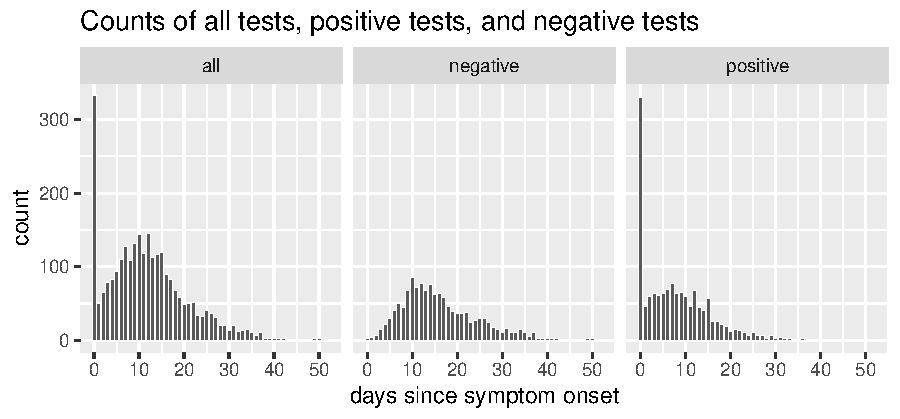
\includegraphics[width=0.35\textwidth]{img/data-counts.pdf}
\end{center}

\section{Unconstrained MLE}

Independent maximum likelihood estimates with $\pm$ standard error
bars.

\begin{center}
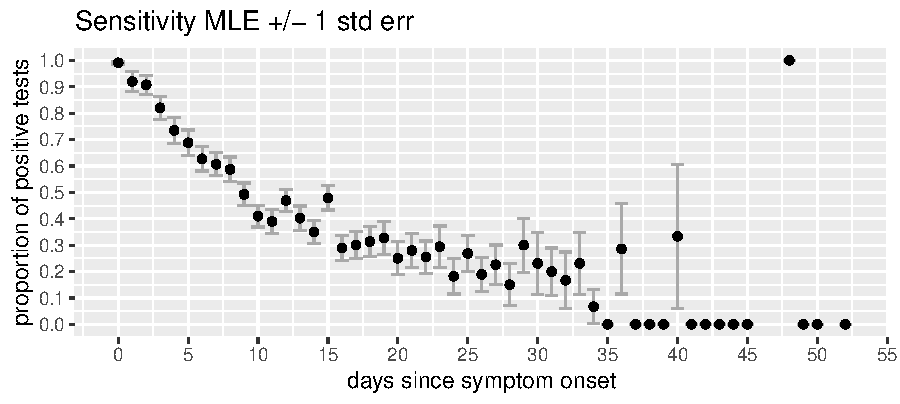
\includegraphics[width=0.35\textwidth]{img/mle.pdf}
\end{center}


\section{Bayesian Models}
\newcommand{\ilogit}{\textrm{logit}^{-1}}

{\bfseries Hetero (logit):} \
$y_n \sim \textrm{bernoulli}(\ilogit(\theta_{t_n}));
\quad \theta_t \sim 
\textrm{normal}(0, 3);
\quad \theta_{t+1} < \theta_t$
\\[12pt]
{\bfseries Hetero (log):} \
$y_n \sim \textrm{bernoulli}(\exp(\theta_{t_n}));
\quad \theta_t \sim \textrm{normal}(0, 3);
\quad \theta_{t+1} < \theta_t < 0$
%
\\ \hrule \mbox{}\\[6pt]
%
{\bfseries RW(1) (logit):} \
$y_n \sim \textrm{bernoulli}(\ilogit(\theta_{t_n}));
\quad \theta_{t+1} \sim \textrm{normal}(\theta_t, \sigma);
\quad \sigma \sim \textrm{normal}(0, 1);$
\\[2pt]
\null\qquad\qquad\qquad\qquad $\theta_{t+1} < \theta_t; 
\quad \sigma > 0$
\\[12pt]
{\bfseries RW(1) (log):} \
$y_n \sim \textrm{bernoulli}(\exp(\theta_{t_n}));
\quad \theta_{t+1} \sim \textrm{normal}(\theta_t, \sigma);
\quad \sigma \sim \textrm{normal}(0, 1);$
\\[2pt]
\null\qquad\qquad\qquad\qquad $\theta_{t+1} < \theta_t < 0;
\quad \sigma > 0$
%
\\ \hrule \mbox{}\\[6pt]
%
{\bfseries RW(2) (logit):} \
$y_n \sim \textrm{bernoulli}(\ilogit(\theta_{t_n})); 
\quad \theta_{t+2} \sim \textrm{normal}(\theta_{t-1} + (\theta_{t-1} - \theta_{t-2}), \sigma);$
\\[2pt]
\null\qquad\qquad\qquad\qquad $\sigma \sim \textrm{normal}(0, 0.5); 
\quad \theta_{t+1} < \theta_t; 
\quad \sigma > 0$
\\[12pt]
{\bfseries RW(2) (log):} \
$y_n \sim \textrm{bernoulli}(\exp(\theta_{t_n})); 
\quad \theta_{t+2} \sim \textrm{normal}(\theta_{t-1} + (\theta_{t-1} - \theta_{t-2}), \sigma);$
\\[2pt]
\null\qquad\qquad\qquad\qquad $\sigma \sim \textrm{normal}(0, 0.5); 
\quad \theta_{t+1} < \theta_t < 0; 
\quad \sigma > 0$
%
\\ \hrule \mbox{}\\[6pt]
%
{\bfseries Regression (logit):} \
$y_n \sim \textrm{bernoulli}(\ilogit(\alpha + \beta \cdot t_n));
\quad \alpha, \beta \sim \textrm{normal}(0, 0.5);
\quad \beta < 0$
\\[12pt]
{\bfseries Regression (log):} \
$y_n \sim \textrm{bernoulli}(\exp(\alpha + \beta \cdot t_n));
\quad \alpha, \beta \sim \textrm{normal}(0, 0.5); \quad \alpha, \beta < 0$
%
\\ \hrule \mbox{}\\[6pt]
%
{\bfseries Regression mix (logit):}
$y_n \sim \textrm{bernoulli}(\ilogit(\lambda \cdot (\alpha_1 + \beta_1 \cdot t_n) + (1 - \lambda) \cdot (\alpha_2 + \beta_2 \cdot t_n)))$
\\[2pt]
\null\qquad\qquad\qquad\qquad $\lambda \sim \textrm{beta}(2, 2);
\quad \alpha_k, \beta_k \sim \textrm{normal}(0, 1);
\quad \beta_k < 0$




\section{Model Comparison}

Approximate leave-one-out cross-validation estimates of expected log
predictive density (ELPD) differences plus standard
errors of differences.  Estimated using Stan's \texttt{loo} package.
\vspace*{12pt}
\begin{center}
\begin{tabular}{ll|rr}
\hline
Model & Scale & ELPD (diff) & standard error (diff)
\\ \hline
2nd-order random walk & \ log &  0.0 & 0.0
\\
Regression mixture & \ log &   -0.4 &      1.5  
\\
1st-order random walk & \ log        &         -0.9 &       0.7  
\\
Regression & \ log &   -2.8  &     2.7  
\\
Heterogeneous & \ log & -3.0     &  1.8  
\\ \hline
Heterogeneous & \ logit &    -3.0    &   1.9  
\\
2nd-order random walk & \ logit  & -6.7     &  3.7  
\\
1st-order random walk & \ logit              & -8.4      & 3.8  
\\
Regresison mixture & \ logit  & -15.0  &     4.1  
\\
Regression & \ logit & -81.6   &    9.9
\\ \hline
\end{tabular}
\end{center}
\end{multicols}
\centering
\vfill
\section{Visual Model Comparison}
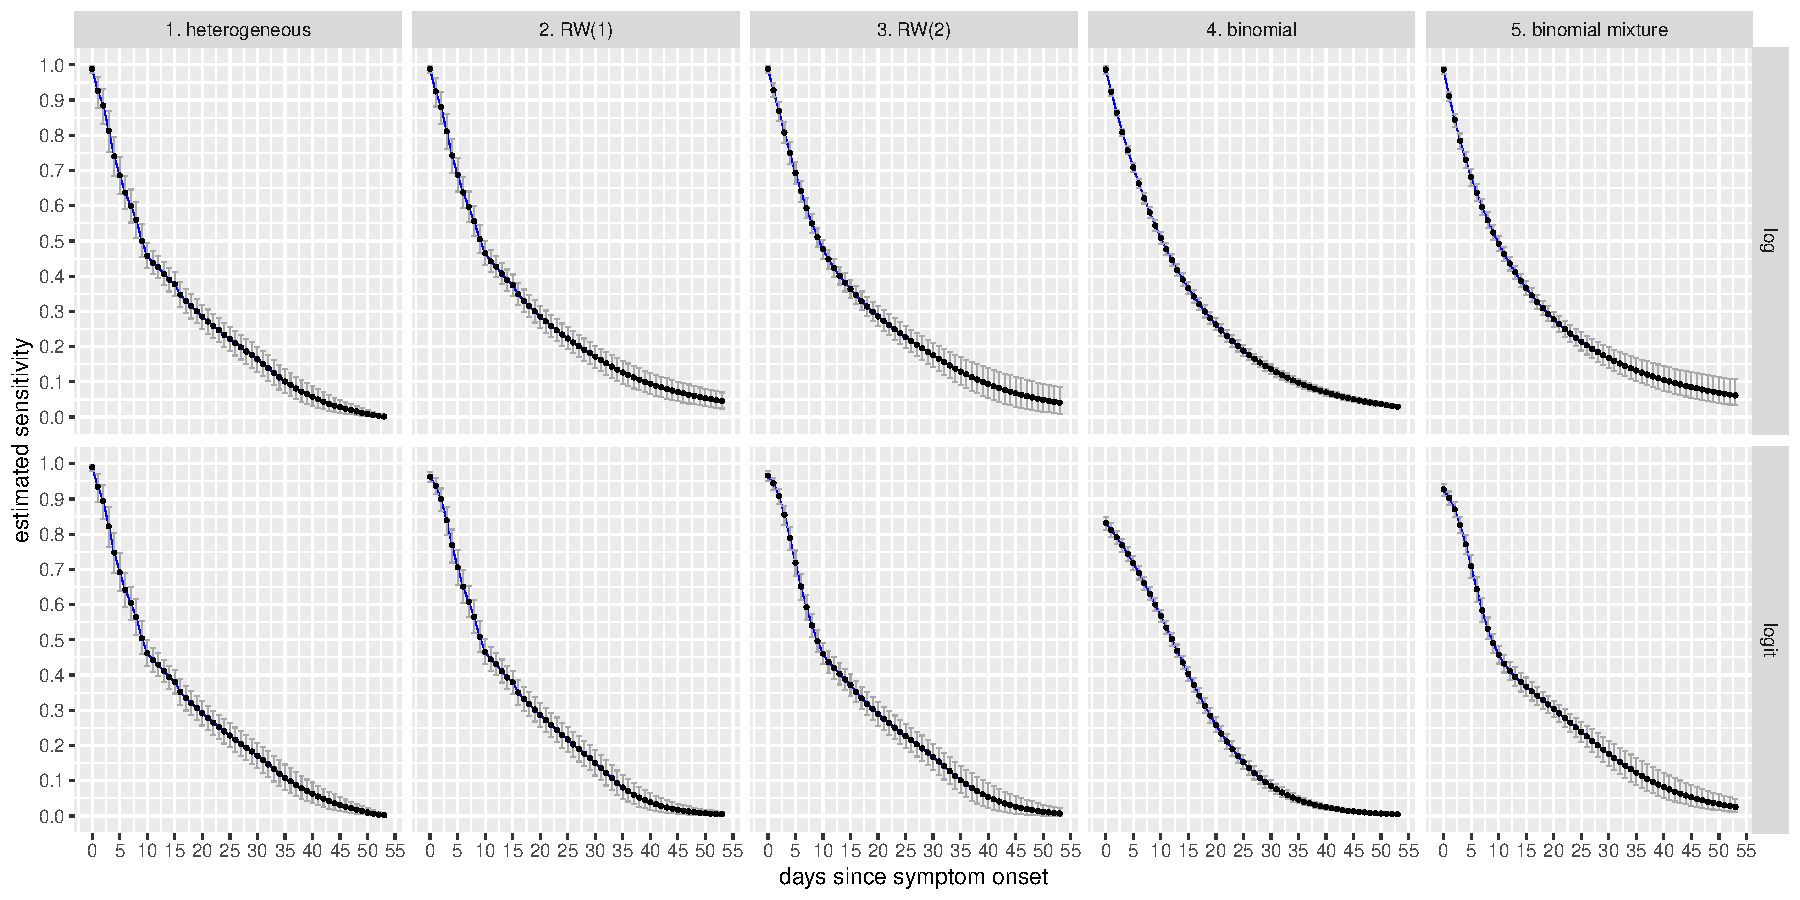
\includegraphics[width=0.8\textwidth]{img/model-link-comparison.pdf}
\end{document}

